\documentclass[conference]{IEEEtran}
\usepackage{cite}
\usepackage{amsmath,amssymb}
\usepackage{hyperref}
\usepackage{graphicx}

\title{RL-Tuned Synthetic Marine Radar for Sim-to-Real Transfer}
\author{\IEEEauthorblockN{Team Name Placeholder} \\
\IEEEauthorblockA{CSCE 775: Deep Reinforcement Learning}}

\begin{document}
\maketitle

\begin{figure*}[t]
\centering
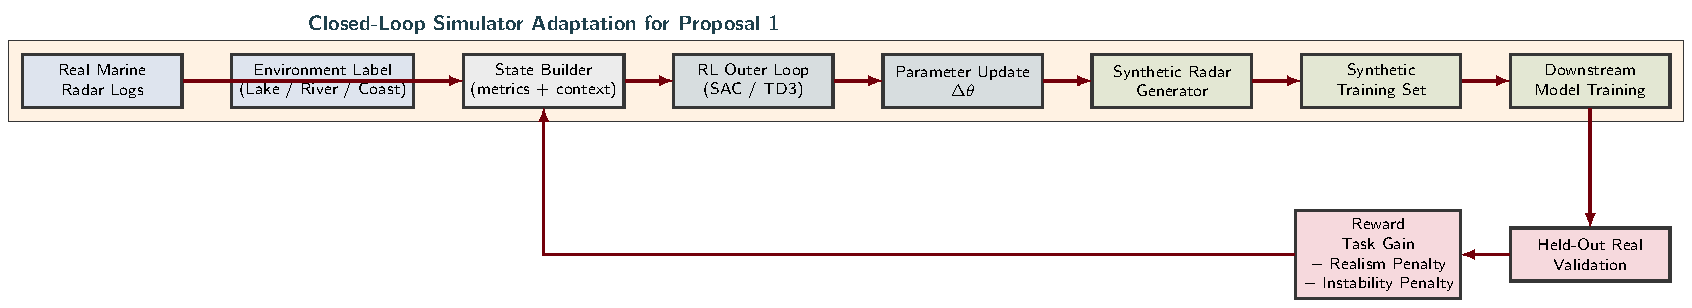
\includegraphics[width=\textwidth]{figures/fig_method_pipeline.pdf}
\caption{Proposal 1 closed-loop method: an RL outer loop updates simulator parameters from real-validation reward, conditioned on environment type.}
\label{fig:method-overview}
\end{figure*}

\begin{figure*}[t]
\centering
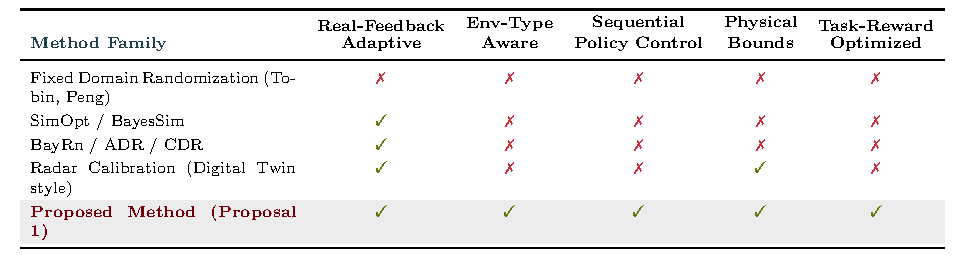
\includegraphics[width=\textwidth]{figures/fig_related_work_matrix.pdf}
\caption{Related-work capability comparison and the explicit improvement axes targeted by Proposal 1.}
\label{fig:rw-matrix}
\end{figure*}

\section{Introduction}
Marine radar is useful for obstacle detection, situational awareness, and local mapping, but robust learning requires large labeled datasets. Because collecting and labeling maritime radar logs is expensive, many pipelines rely on synthetic data. This creates a persistent sim-to-real gap: models that perform well in simulation can degrade substantially on real sensor data.

This proposal asks whether simulator parameters can be tuned automatically so synthetic training distributions better match real maritime operating regimes. We study an RL controller that updates simulator parameters to maximize held-out real-validation performance. The controller is conditioned on broad environment type (`lake`, `river`, `coast`) with the hypothesis that context-aware tuning outperforms fixed settings and uniform randomization, especially under route and clutter shift.

The method builds on domain-randomization and adaptive sim-to-real literature \cite{tobin2017domain,peng2018sim,chebotar2018simopt,ramos2019bayessim,muratore2020bayrn,openai2019rubik,josifovski2024cdr,ho2020rap,zhao2020sim2real}. Radar transfer motivation is further supported by recent radar-domain studies \cite{kim2024soft,trinh2026digitaltwin} and by public real-radar datasets that expose weather and domain shift challenges \cite{sheeny2020radiate,ouaknine2020carrada,schumann2021radarscenes,choi2024polaris,zust2023lars}. Prior work often uses fixed/random perturbations, one-shot adaptation, or calibration pipelines without explicit maritime context. Our contribution is an environment-aware RL outer loop that optimizes downstream real-task reward directly (Fig.~\ref{fig:method-overview}) and is compared against explicit capability gaps in related work (Fig.~\ref{fig:rw-matrix}).


\section{Approach}
We cast simulator tuning as a bi-level optimization problem. Let $\mathcal{M}$ be the downstream perception model (e.g., MRISNet for ship segmentation \cite{ma2024mrisnet}) and $\mathcal{S}(\theta, e)$ be a physically grounded radar simulator parameterized by $\theta$ and conditioned on environment type $e \in \{\text{lake}, \text{river}, \text{coast}\}$. The objective is
\begin{equation}
    \theta^* = \arg\max_{\theta} \mathcal{R}\left(\mathcal{M}^*(\theta), \mathcal{D}_{real}\right)
\end{equation}
subject to inner-loop training
\begin{equation}
    \mathcal{M}^*(\theta) = \arg\min_{\omega} \mathcal{L}_{task}\left(\mathcal{M}_{\omega}, \mathcal{S}(\theta, e)\right).
\end{equation}

The outer-loop policy $\pi(\theta_{t+1} \mid s_t)$ proposes sequential updates to simulator parameters. State $s_t$ includes current $\theta$, environment label $e$, recent validation metrics, and trajectory history. Reward is
\begin{equation}
    r_t = \Delta \mathrm{mIoU}_{real} - \lambda_1\|\theta_t-\theta_{init}\|_2 - \lambda_2\,\mathbb{1}(\theta \notin \Omega_{phys}),
\end{equation}
where $\Omega_{phys}$ denotes physically plausible bounds.

The simulator models multipath and clutter using physically meaningful factors: speckle scale, attenuation, clutter floor, and multipath gain. To avoid unrealistic exploitation, each action is clipped to calibrated parameter ranges and penalized when violating physical plausibility. We use Soft Actor-Critic (SAC) for the outer loop because it supports stable learning in continuous action spaces with stochastic exploration.

The key design difference from prior adaptive randomization is that this policy is (i) sequential, (ii) environment-conditioned, and (iii) optimized on downstream real-task reward rather than simulator similarity alone.


\begin{figure*}[t]
\centering
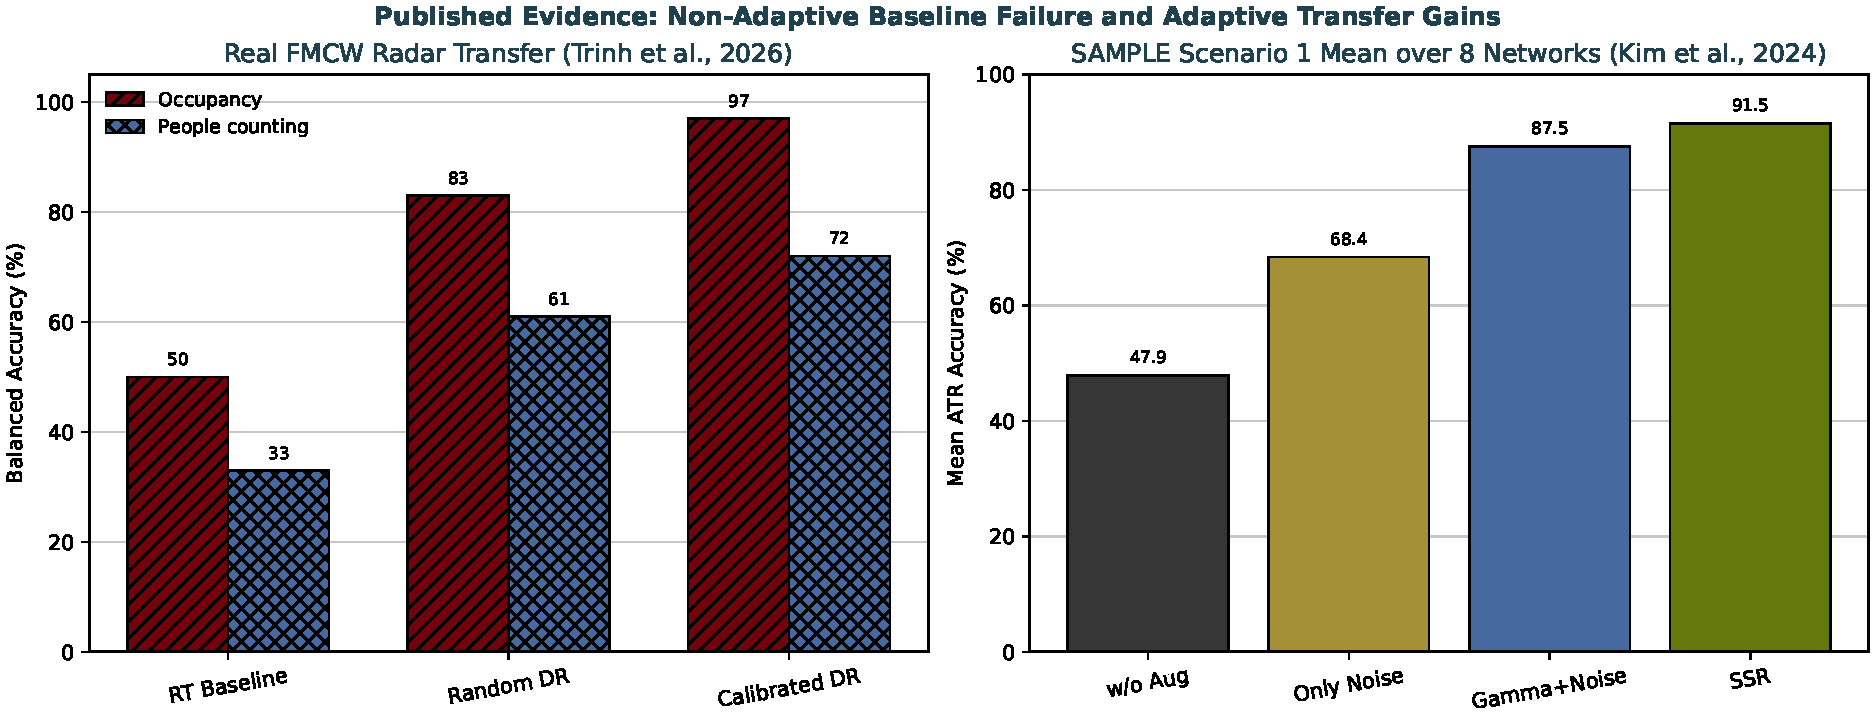
\includegraphics[width=\textwidth]{figures/fig_published_evidence_results.pdf}
\caption{Published quantitative evidence motivating Proposal 1. Left: non-adaptive and weakly adaptive baselines can fail under sim-to-real radar transfer; calibrated/adaptive methods improve substantially. Right: synthetic-only and simple noise baselines underperform on measured-data transfer compared to stronger adaptation strategies.}
\label{fig:published-evidence}
\end{figure*}

\section{Evaluation}
Evaluation uses real marine radar logs from the MOANA \cite{moana2025} and PoLaRIS \cite{choi2024_polaris} datasets, featuring explicit environment labels and strict splits by route/location to avoid leakage. We employ MRISNet \cite{ma2024_mrisnet} as the primary downstream perception model to evaluate ship instance segmentation performance. We compare five settings: (1) fixed simulator defaults, (2) uniform random domain randomization, (3) Bayesian optimization tuning, (4) RL tuning without environment labels, and (5) RL tuning with environment labels.

The primary outcome is real-data task performance and corresponding reduction in sim-to-real gap. Secondary outcomes are cross-domain generalization (train on two environment types, test on the held-out type), robustness on unseen locations, run-to-run variance, and behavior under low-SNR/high-clutter stress tests. We also report sample efficiency as the number of real-validation calls needed to reach a target accuracy.

Each novelty claim is tied to a direct test: (a) benefit of sequential RL adaptation versus BayRn under matched evaluation budgets \cite{muratore2020bayrn}; (b) benefit of environment semantics via conditioned versus unconditioned RL; and (c) benefit of physical realism constraints via bound-violation and instability rates with/without realism regularization. This structure makes it explicit how the proposed method differs from existing randomization and adaptation families \cite{tobin2017domain,peng2018sim,chebotar2018simopt,ramos2019bayessim,openai2019rubik,josifovski2024cdr}.

Prior published results already motivate this direction (Fig.~\ref{fig:published-evidence}). In real FMCW transfer, simulation-only baselines can approach chance-level behavior, while calibrated adaptation improves substantially \cite{trinh2026digitaltwin}. In synthetic-to-measured SAR transfer, synthetic-only and simple-noise baselines are again weaker than stronger adaptation methods \cite{kim2024soft}. Together, these patterns motivate structured, feedback-driven simulator control rather than fixed randomization.


\section{Conclusion}
This project targets a practical problem with broad relevance beyond radar: models trained in simulation often fail when deployed in the real world. We propose an environment-aware RL controller that tunes synthetic data generation to improve real-data task performance, and we benchmark it against strong non-RL alternatives under realistic transfer stress tests. If full RL tuning is unstable, a contextual-bandit or Bayesian fallback still yields a complete and informative outcome.


\bibliographystyle{IEEEtran}
\bibliography{../bibliography/references}

\end{document}
